\subsection{System Controlling}\label{ssec:mcu-review}
	In order to automate break tests a system block that should be able to interface both sensor signals and user commands to the system is needed. Summarizing, this block should be responsible to handle the interface between the electric signals and higher level user instructions.
	\par
	At the design of this block of the solution a important thing should be considered, data acquisition. According to \cite{ni-daq} DAQ (Data Acquisition) can be defined as the process of measuring an electric or physical phenomenon, such as voltage, current, temperature, pressure or sound.
	\par
	As mentioned in Section \ref{sec:purpose}: \textit{"The system should be able to perform brake tests by controlling the mechanical parts while acquiring relevant data with the aid of sensors and transducers"}. There is a type of device that is able to perform data acquisition and system control, the microcontroller.

	\subsubsection{Microcontroller basic characteristics}\label{sssec:microcontroller-basic-characteristics}

		A microcontroller is a compact computer on a single integrated circuit chip, in most cases a microcontroller (also refered by the acronym MCU) includes a processor, volatile and non-volatile memory, input/output ports and other peripherals. The great thing about the microcontrollers is their low cost, many small appliances that does not require a powerful hardware are only economically viable because of those devices. The components a microcontroller has may vary, it is a responsability of the project designer to decide the microcontroller that has the best fit (technically and economically) for the project.
		\par
		Microcontrollers differ from microprocessors only in one thing, MCUs can be used standalone while microprocessors need other peripherals to be used. By reducing the size and cost compared to a design that uses a separate microprocessor, memory, and input/output devices, microcontrollers make it economical to digitally control even more devices and processes. \say{A microprocessor can be considered the heart of a computer system, whereas a microcontroller can be considered the heart of an embedded system}\cite{mcuDef}.
		\par
		A great thing about microcontrollers is that they can provide provide real-time response to events, so for instrumentation they are crucial. With them it is possible to acquire signals with good sampling rates without loss of relevant information \cite{bartz2004data}.

	\subsubsection{Microcontroller Architecture and Most Important Parts}\label{sssec:microcontroller-architecture-and-most-important-parts}

		In order to understand how a typical MCU parts are, Figure \ref{fig:atmega32u4-architecture} show the block diagram of the ATmega32U4, a MCU manufactured by Microchip.

	\begin{figure}[htbp]
		\centering
			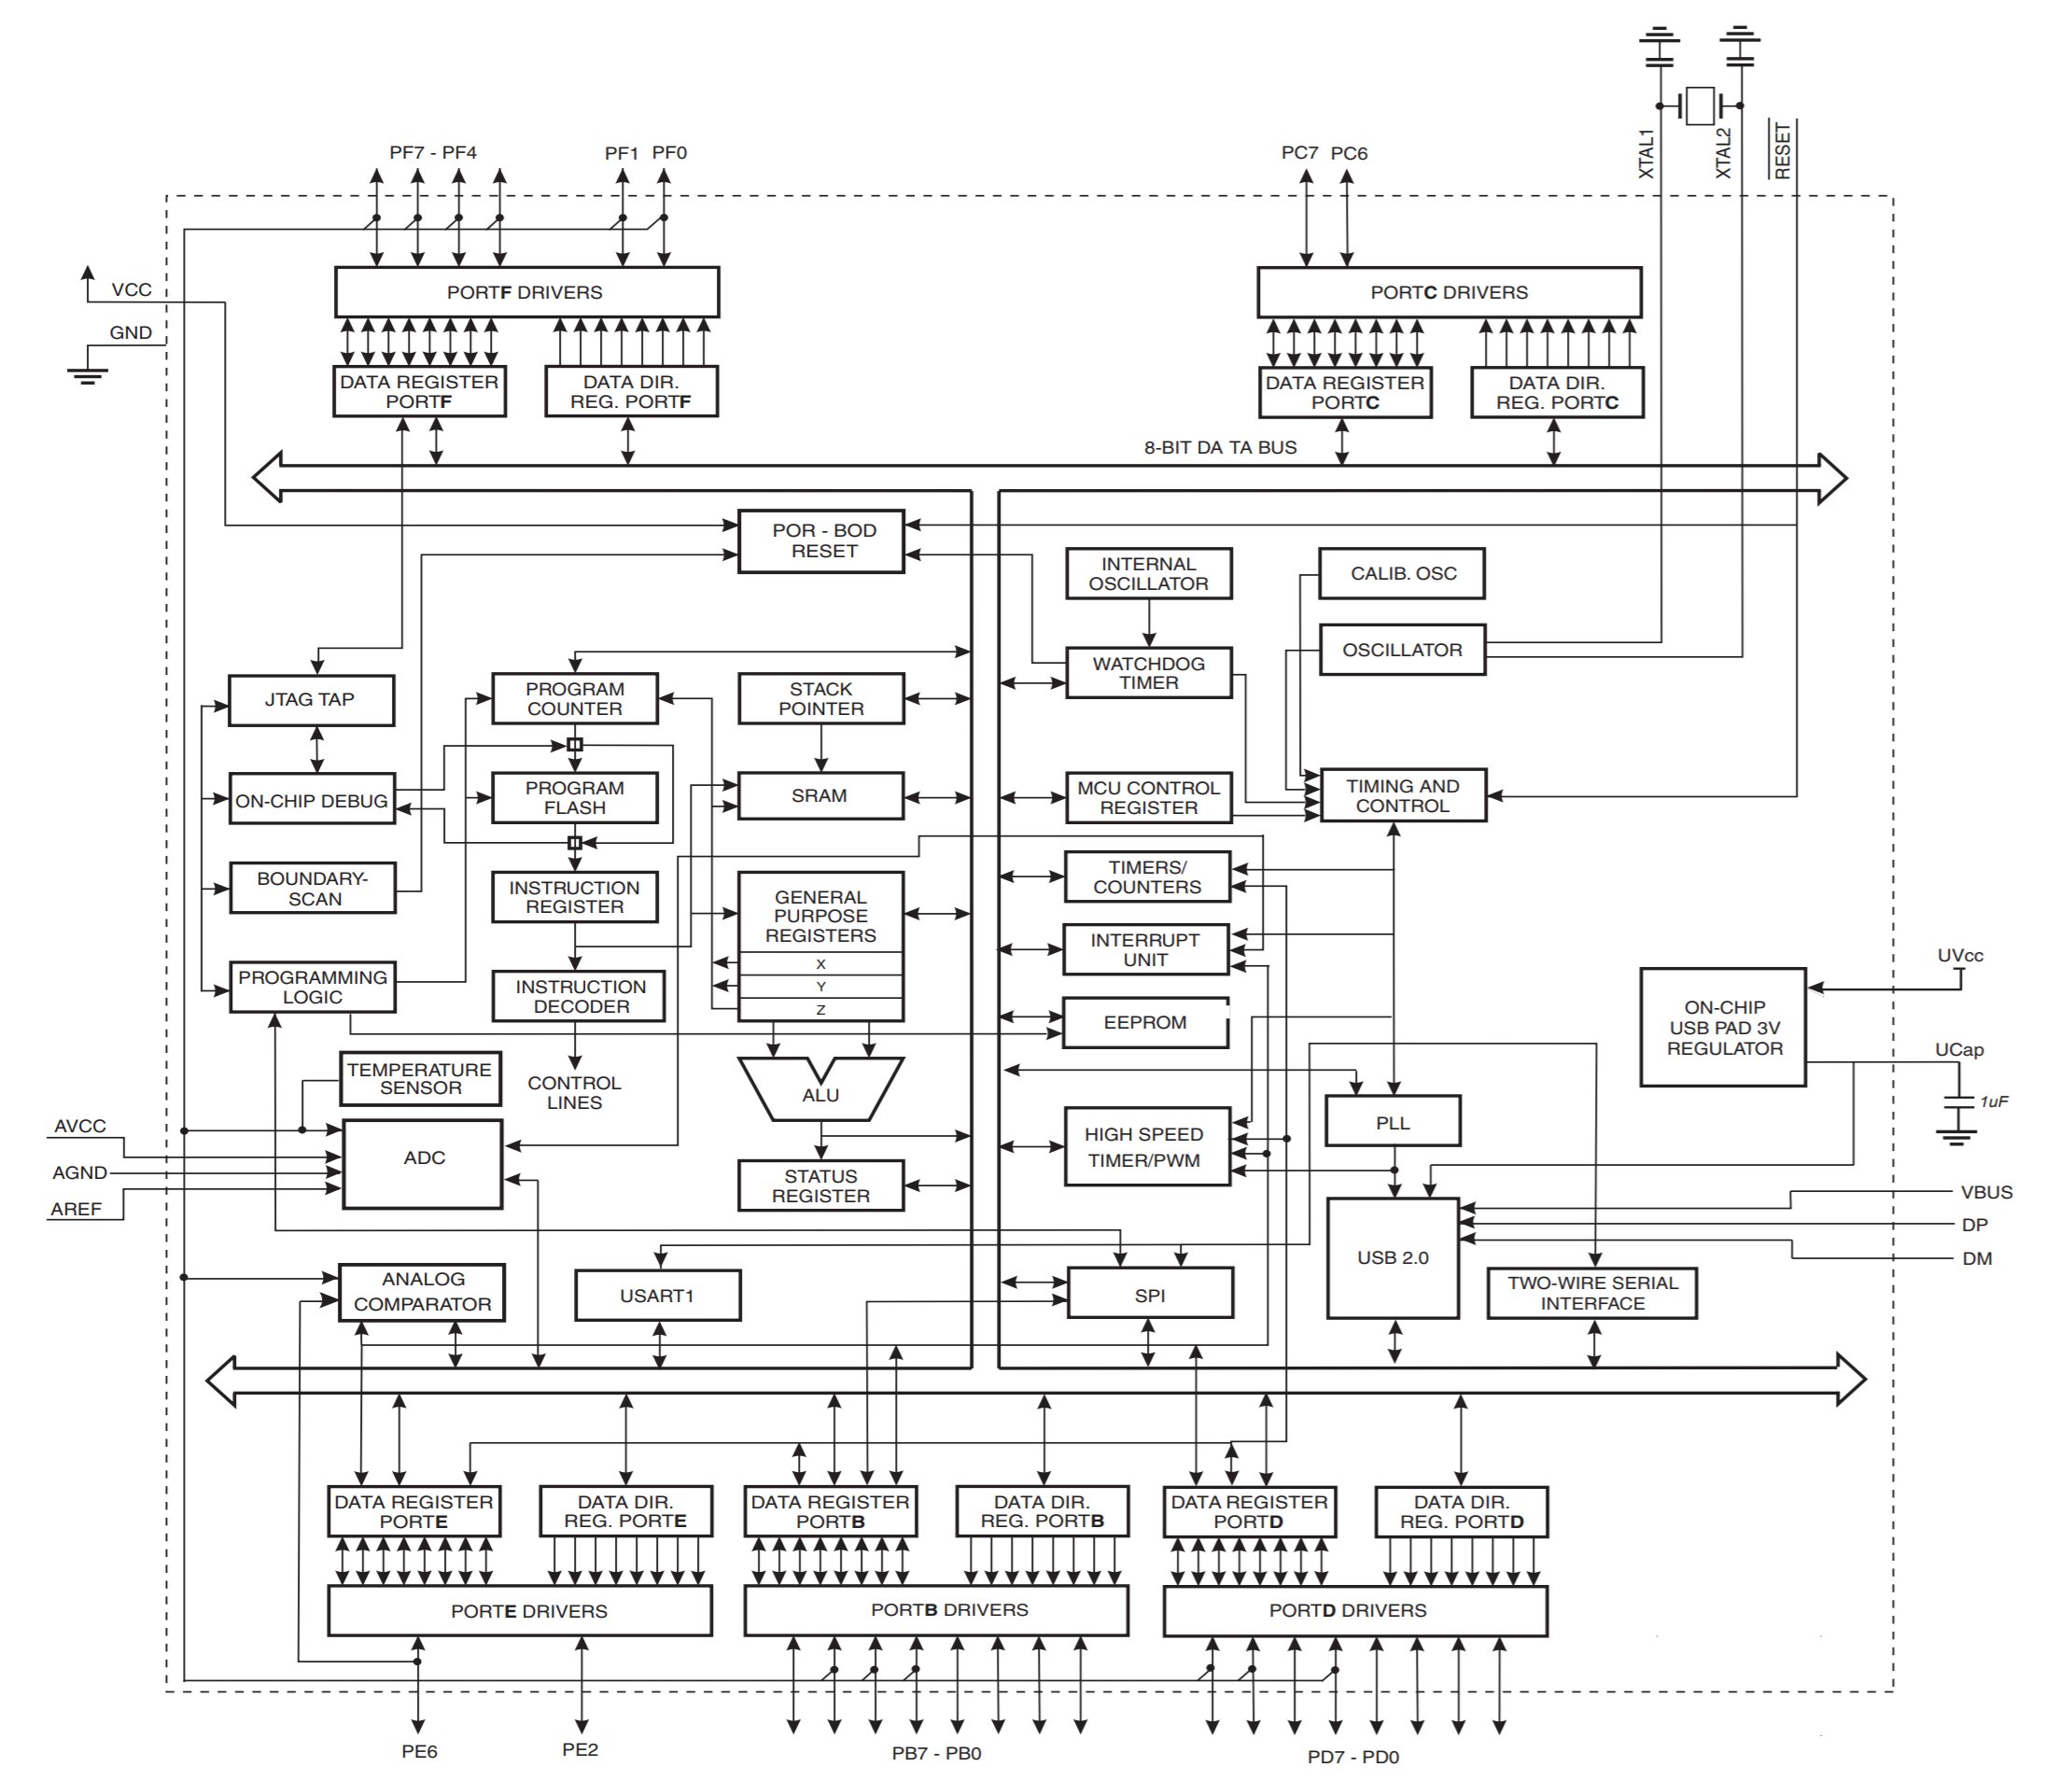
\includegraphics[width=1\textwidth]{figuras/fig-atmega32u4-architecture}
		\caption{ATmega16/32U4 Block Diagram \cite{atmega32u4-architecture}}
		\label{fig:atmega32u4-architecture}
	\end{figure}

		The most important blocks of this device are:

		\begin{itemize}
			\item\textit{Timing and Control}: This circuit block represents the part of MCU responsible for maintaing the clock signals and handle time events.\label{itm:timing-and-control}
			\item\textit{Program Flash}: This is a non-volatile memory used to store the code, MCUs can execute code directly from the flash memory.\label{itm:program-flash}
			\item\textit{Port Drivers}: This are the device \textit{I/Os (inputs/outputs)}, they can be digital or analog ports (execpt for outputs which can only be digital).\label{itm:port-drivers}
			\item\textit{ADC (Analogic to Digital Converter)}: MCUs are by nature digital devices, when acquiring a analog signal, they first make a conversion to a digital value and then copy this data to a register.\label{itm:adc}
			\item\textit{USB 2.0}: Although not being a common feature, some MCUs include a USB (Universal Serial Bus) port. When interfacing with other USB devices, already having this feature inside the MCU saves space and costs when integrating the MCU in a circuit board.\label{itm:mcu-usb}
			\item\textit{High Speed Timer/PWM}: As mentioned in Item \ref{itm:port-drivers}, MCUs do not have analog outputs, the high speed is used to generate a special digital output signal which will be explained on Section \ref{ssec:mcu-pwm}.\label{itm:high-speed-timer-pwm}
		\end{itemize}

	\subsubsection{Pulse Width Modulation} \label{ssec:mcu-pwm}
	Pulse Width Modulation (PWM), is a way of modulation for encoding information on a digital pulse train signal. There are many ways of encoding and extracting this message in and out of the PWM signal and this type of modulation can be used for a wide varriety of applications such as controlling the charge delivered to a load and transmitting information \cite{standard19961037c}. PWM signals have a fixed high and a fixed low voltage level, there are two parameters that can be varried on a PWM signal: oscilation frequency and duty cycle. Figure \ref{fig:dutyCycle} shows how a the duty cycle affects a PWM signal. 

	\begin{figure}[htbp]
		\centering
			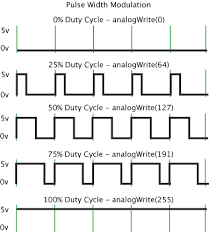
\includegraphics[width=.45\textwidth]{figuras/fig-dutyCycle}
		\caption{Duty Cycle Examples \cite{fig-dutyCycle}}
		\label{fig:dutyCycle}
	\end{figure}

	Duty cycle can be defined mathematically by the Equation \ref{eqn:dutyCycle} \cite{james2001fundamentals}, where \textit{$D_{\%}$} is the duty cycle in percentage, \textit{PW} is the pulse width (pulse active time) and \textit{T} is the wave period. 

	\begin{equation}\label{eqn:dutyCycle}
		D_{ \left( \% \right) } =\frac{PW}{T}
	\end{equation}

	One useful way of using a PWM duty cycle variation is by enconding a analog voltage level proportional into it's percentage \cite{holmes2003pulse}, meaning that 100$\%$ duty cycle would represent maximum voltage amplitude and 0$\%$ the minimum voltage. This means it is possible to extract a analog voltage level by taking a PWM average level \cite{alter2008pwm}, this is a practical way for designing digital to analog converters.

\begin{comment}
	\subsubsection{Microcontroller ISP programming}\label{sssec:microcontroller-isp-programming}

		In-system programming (ISP), also called in-circuit serial programming (ICSP), is a technique where a programmable device is programmed after the device is placed in a circuit board \cite{icsp-guide} rather than before placing the circuit in the board.
		\par
		There are many different standards protocols for ISP, most of them variants from the Joint Test Action Group (JTAG) protocol \cite{oshana2002introduction}. An example of devices using ISP is the AVR line of micro-controller by Microchip such as the ATmega328PB MCU \cite{atmega328p-datasheet}. According to \cite{equinox-isp}, important ISP definitios are:

		\begin{itemize}
			\item\textit{\textbf{ISP Programmer:}} This is a device which is capable of producing the required logic and power signals to in-system program the \textbf{\textit{Target Microcontroller}}.\label{itm:isp-programmer}
			\item\textit{\textbf{Target Microcontroller:}} This is the MCU which is to be in-system programmed.\label{itm:isp-target-mcu}
			\item\textit{\textbf{Target System:}} The Target System is the physical PCB which contains the MCU to be in-system programmed.\label{itm:isp-target-system}
			\item\textit{\textbf{ISP Header:}} The programmer must interface to the correct pins of the target device, systems that have ISP programmers usually have a standard connector to ensure the connection is done the right way between the programmer and the MCU.\label{itm:isp-header}
		\end{itemize}

		Figure \ref{fig:typical-connections-for-isp-programming} show the typical connection for most AVR ISP systems

			\begin{figure}[htbp]
				\centering
				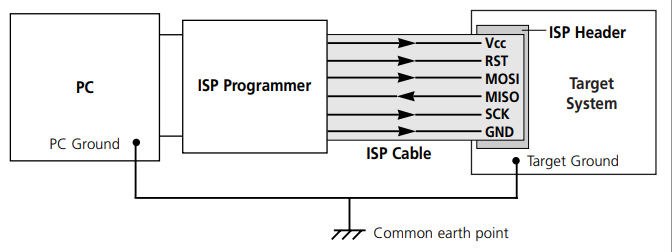
\includegraphics[scale=0.7]{figuras/fig-typical-connections-for-isp-programming.png}
				\caption{Typical Connections for ISP Programming \cite{typical-connections-for-isp-programming}}
				\label{fig:typical-connections-for-isp-programming}
			\end{figure}


		According to \cite{equinox-isp}, the signals from the 6-pin headers are:

		\begin{itemize}
			\item\textit{\textbf{VCC: }} Programmer Vcc Connection.\label{item:isp-vcc}
			\item\textit{\textbf{MOSI: }} Programmer MOSI signal (SPI Data Out).\label{item:isp-mosi}
			\item\textit{\textbf{MISO: }} Programmer MISO signal (SPI Data In).\label{item:isp-miso}
			\item\textit{\textbf{RESET: }} Programmer RESET Control Line.\label{item:isp-reset}
			\item\textit{\textbf{GND: }} Programmer Ground Connection.\label{item:isp-gnd}
			\item\textit{\textbf{SCK: }} Programmer Serial Clock Signal.\label{item:isp-sck}
		\end{itemize}}
\end{comment}